\chapter{Modelo de predição de óbitos proposto}
\label{cap:modelo}

\section{Descrição do dataset utilizado}

Os inputs utilizados no modelo de predição correspondem aos mesmos utilizados nos gráficos da seção \ref{cap:background} deste estudo, porém foram submetidos a diferentes procedimentos de preparação.

As tabelas foram retiradas do site \textit{OpenDataSus} e Coronavírus Brasil. O \textit{OpenDataSus} reúne conjuntos de informações governamentais coletados em colaboração com as secretarias de saúde estaduais, enquanto o Coronavírus Brasil disponibiliza os mesmos dados de forma mais processada.

Especificamente, os números de vacinação foram extraídos do conjunto "Campanha Nacional de Vacinação contra Covid-19" no \textit{OpenDataSus}. Por outro lado, as estatísticas diárias de casos novos e óbitos foram retiradas do site Coronavírus Brasil.

O intervalo de dados abrange janeiro de 2020 a dezembro de 2022. Antes da análise, realizou-se um pré-processamento que incluiu a substituição dos valores faltantes por zero e a agregação das datas em intervalos mensais e anuais.

As tabelas resultantes são organizados em uma matriz de 36 linhas (representando o período de 01/01/2020 a 31/12/2022) e 3 colunas (indicando a quantidade de vacinados, casos novos e óbitos). Esses dados foram usados tanto para os gráficos da seção \ref{cap:background}, que focam na Região Centro-Oeste, quanto para o modelo de predição, onde o foco é o Estado de Goiás.

\section{Descrição do modelo aplicado}

Observando os modelos do mapeamento sistemático realizado na seção \ref{cap:mapeamento} deste trabalho, o modelo LSTM foi utilizado em dois dos seis artigos analisados, e obteve um bom resultado na predição, portanto o algoritmo de predição é no modelo LSTM.

Por se tratar de uma tabela pequena , foi utilizado o modelo mais simples que é o sequencial. O \textit{target} foi a coluna de quantidade de óbitos e as \textit{features} a quantidade de casos novos e a quantidade de doses.

\begin{table}[ht]
    \centering
    \begin{tabular}{|c|c|}
    \hline
         \textbf{Parâmetros} & \textbf{Valores} \\
         \hline
         Números de camadas & 3 \\
         \hline
         Números de nós em cada camada & 40, 40 \\
         \hline 
         Números de camadas completamente conectadas & 1 \\
         \hline
         Número de nós em camadas completamente conectadas & 1 \\
         \hline
         Tamanho do lote & 5 \\
         \hline
         Épocas & 50 \\
         \hline
    \end{tabular}
    \caption{Parâmetros usados no modelo de predição LSTM}
    \label{tab:my_label3}
\end{table}

\section{Avaliação experimental}

O resultado apresenta um \textit{overfitting} dos dados, sendo incapaz de predizer os próximos valores. A média de perda é de $0,035$ nos dados de treinamento e o $R^{2}$ \textit{score} na validação é menor que $-1$. 

\begin{figure}[!ht]
    \centering
    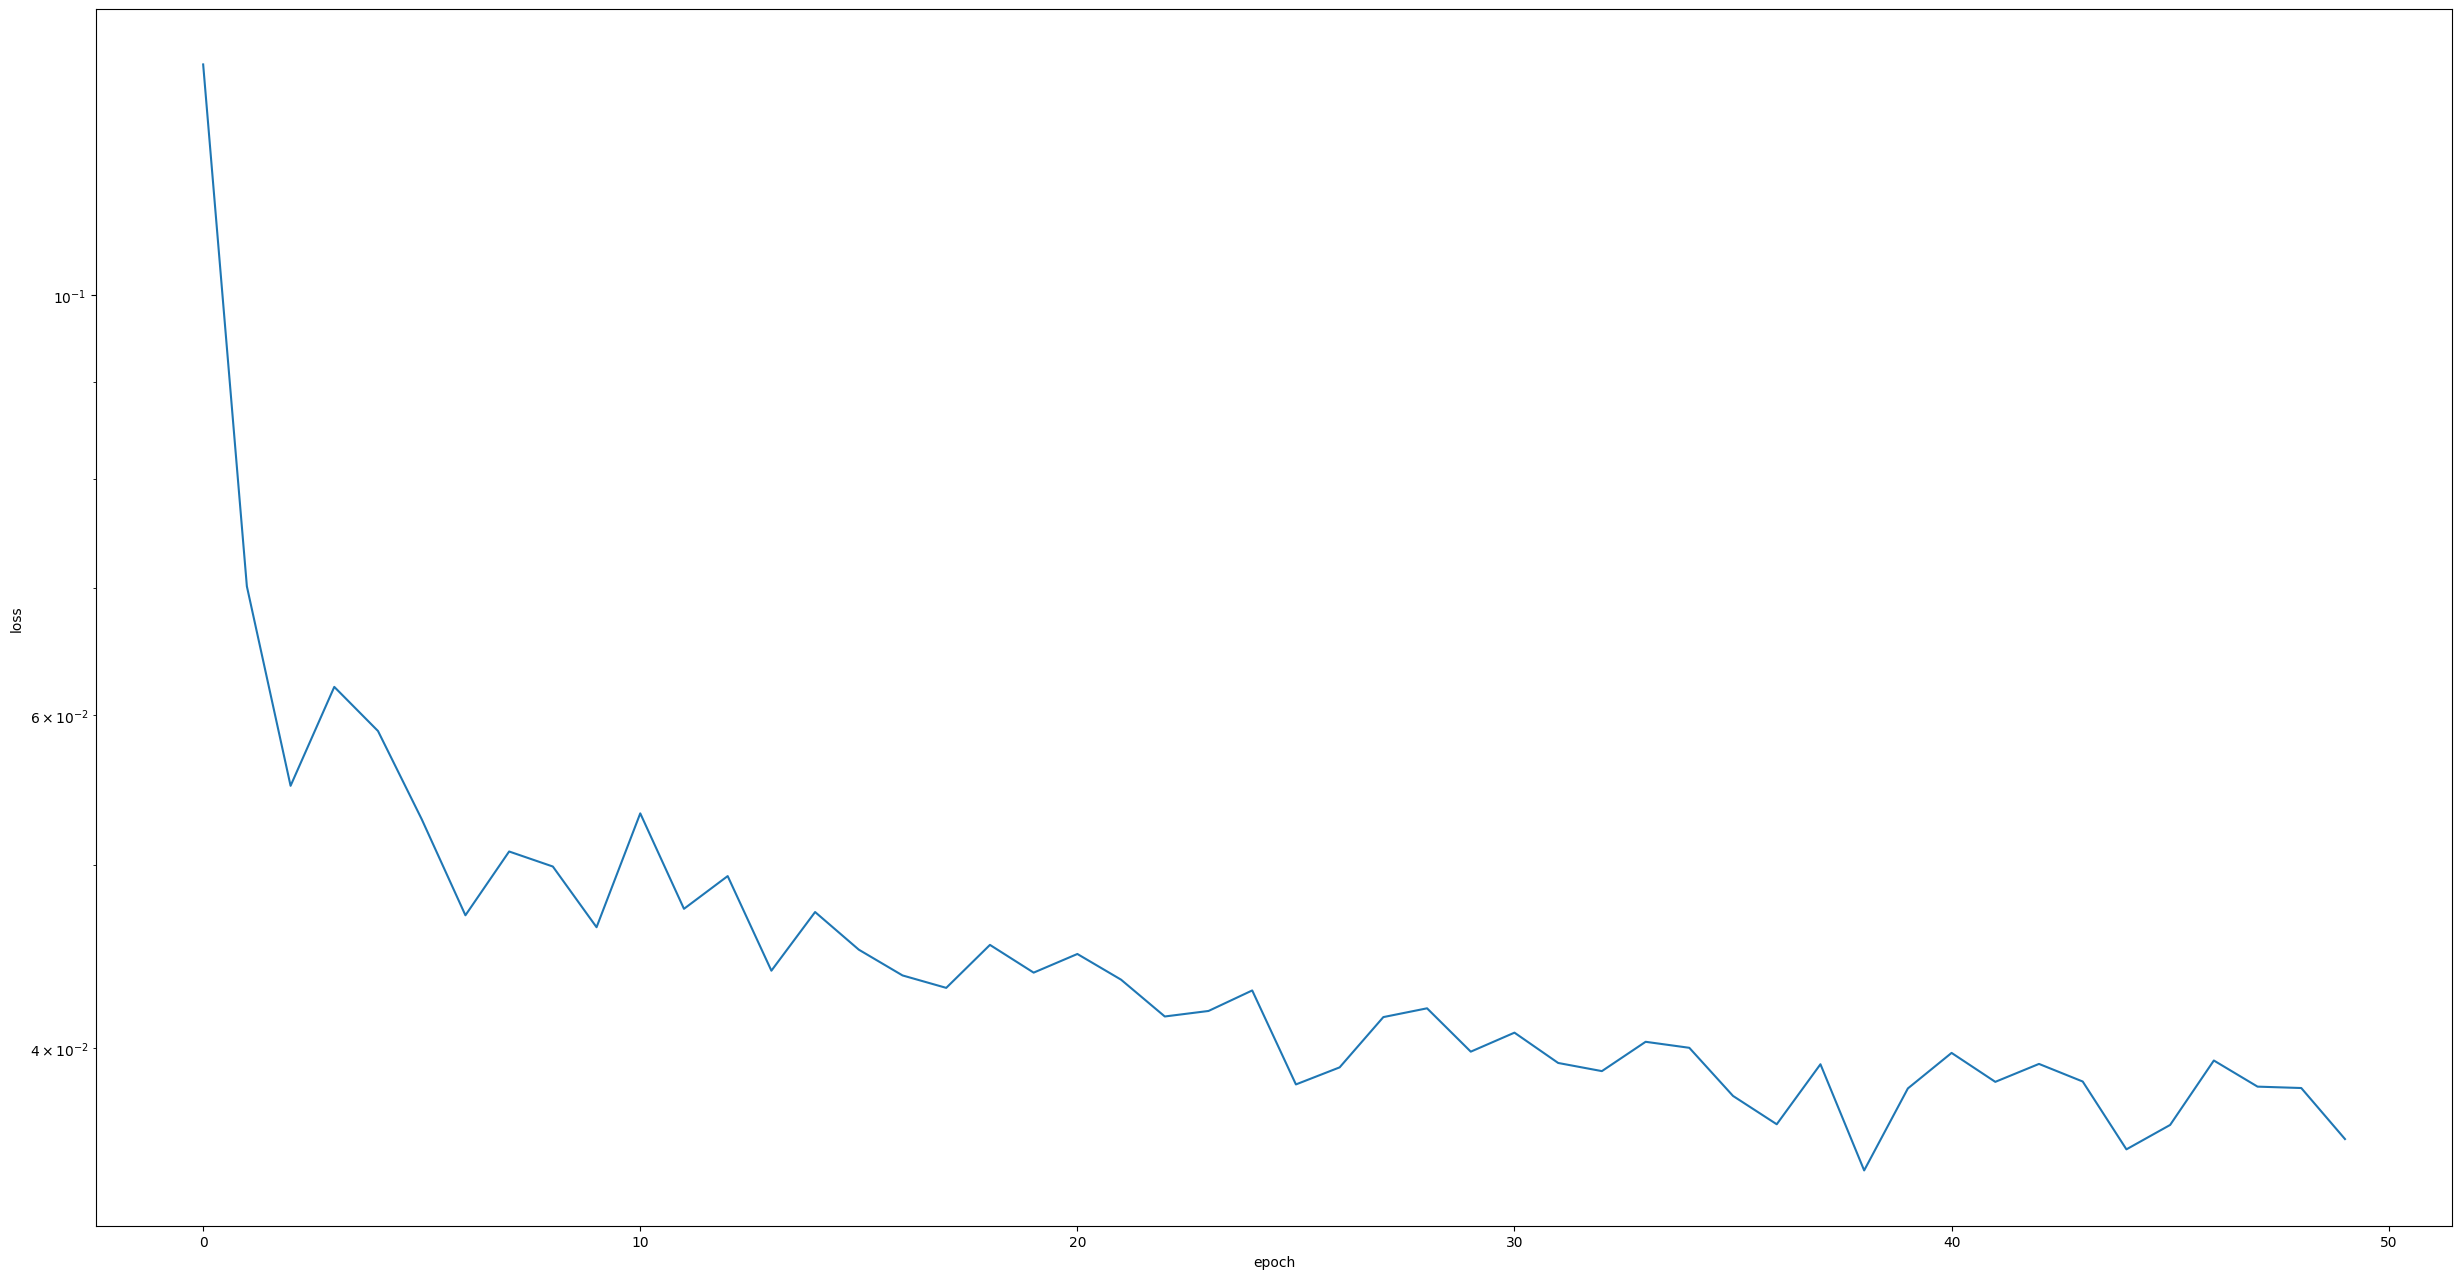
\includegraphics[width=0.99\linewidth]{fig/ModeloLSTM/treinamento.png}
    \caption{Gráfico gerado na fase de treinamento da LSTM}
    \label{fig:enter-label41}
\end{figure}

\begin{figure}[!ht]
    \centering
    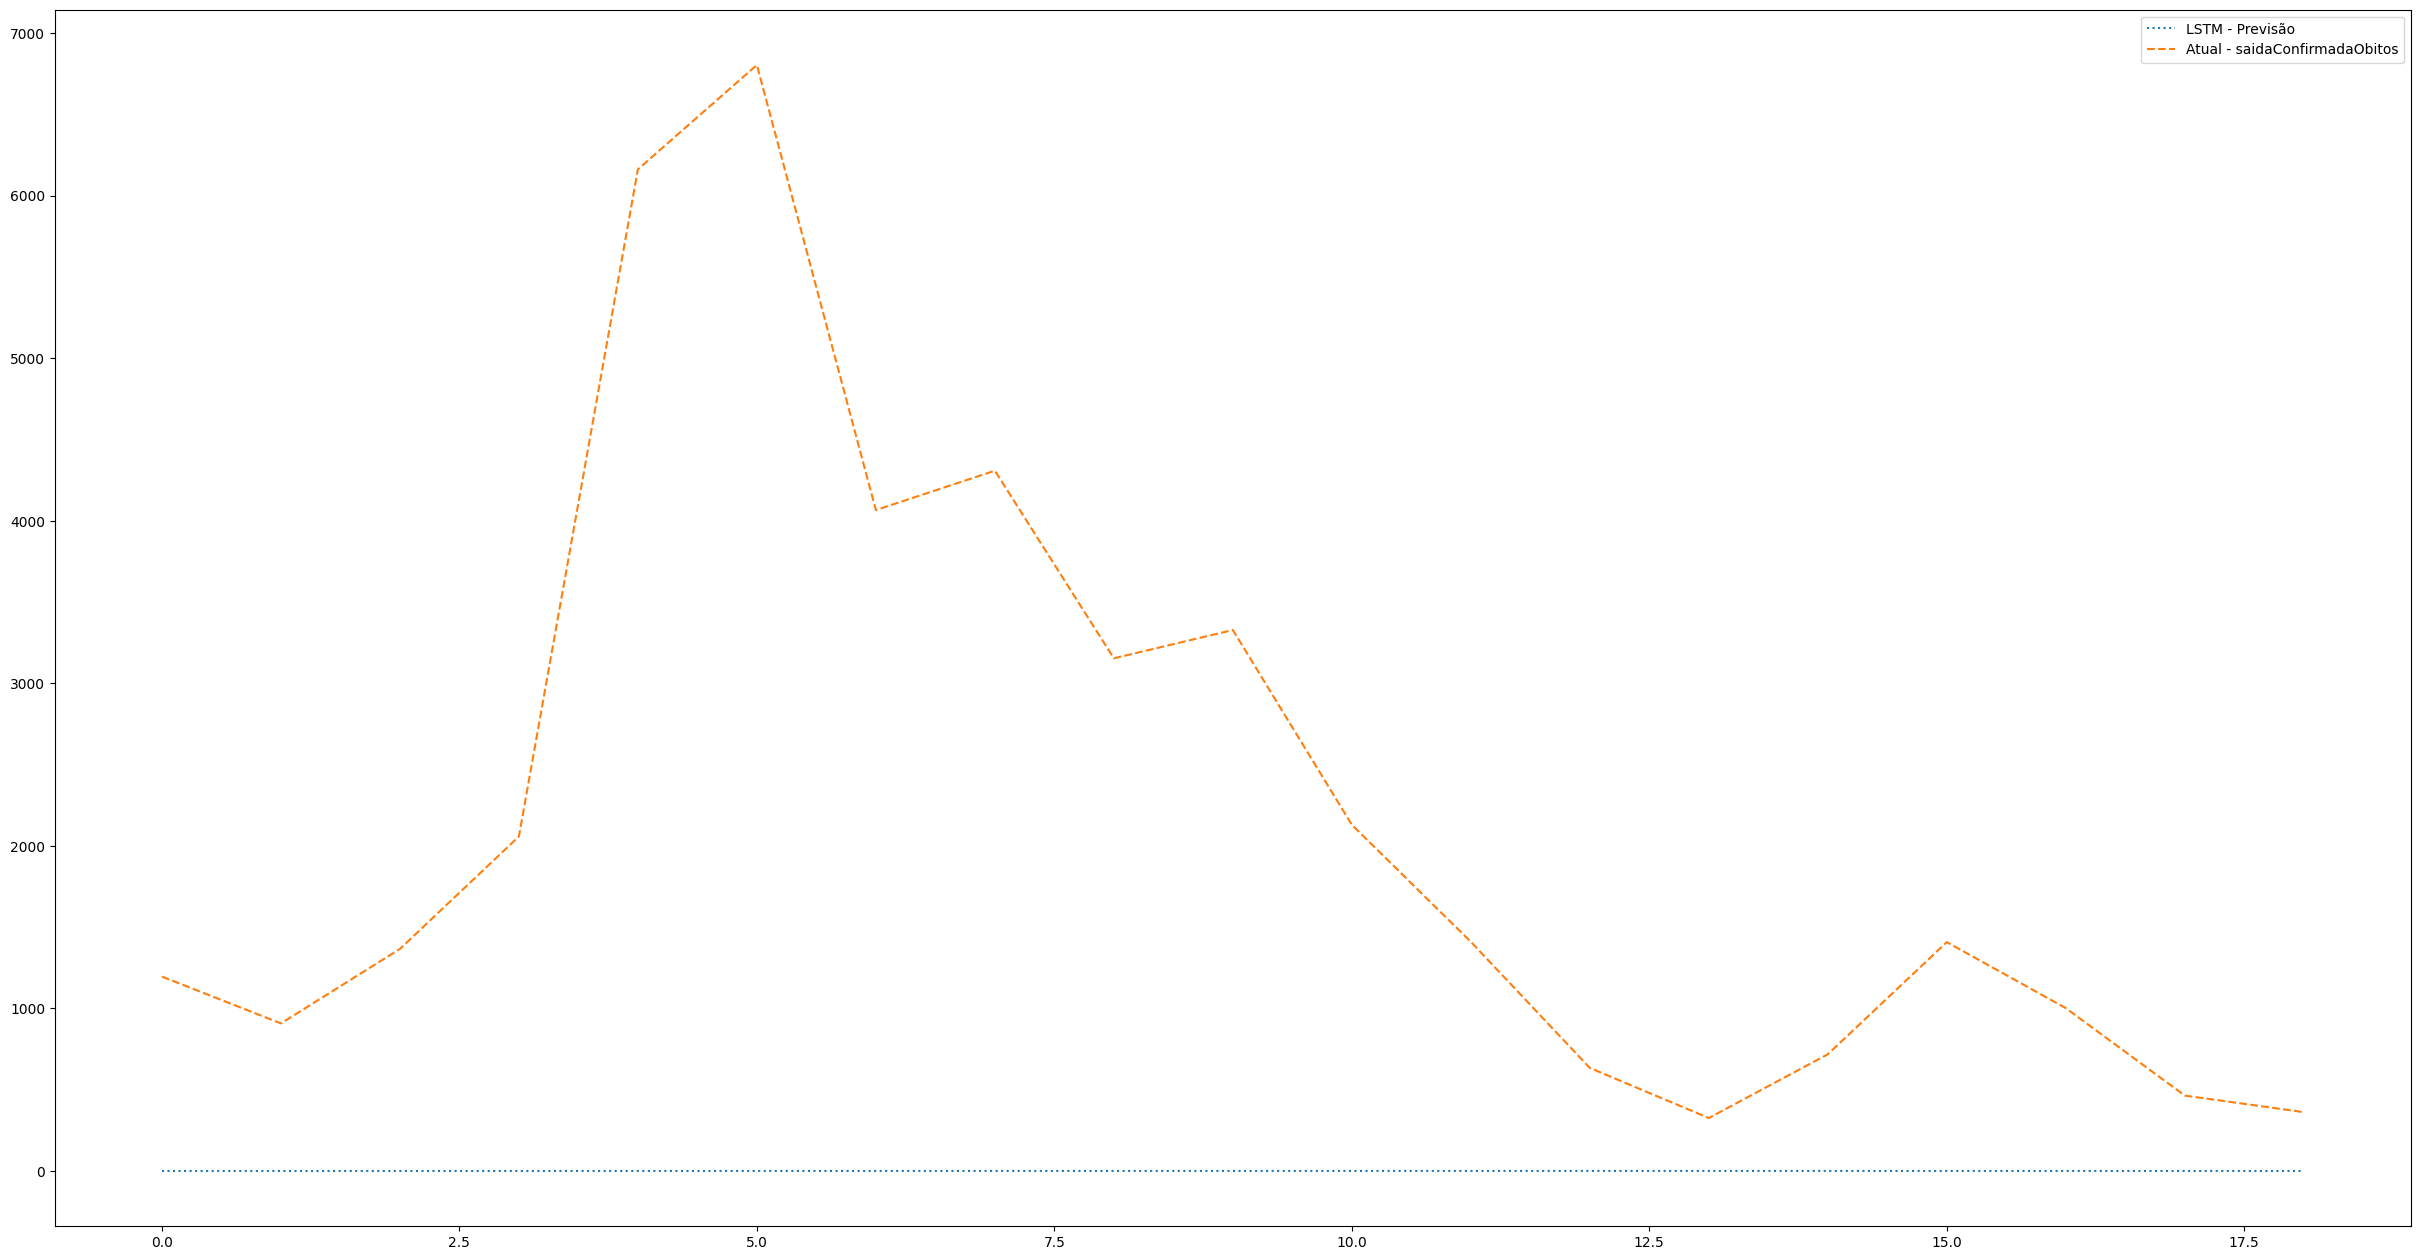
\includegraphics[width=0.99\linewidth]{fig/ModeloLSTM/validacao.png}
    \caption{Gráfico gerado na fase de validação da LSTM}
    \label{fig:enter-label42}
\end{figure}

\begin{figure}[!ht]
    \centering
    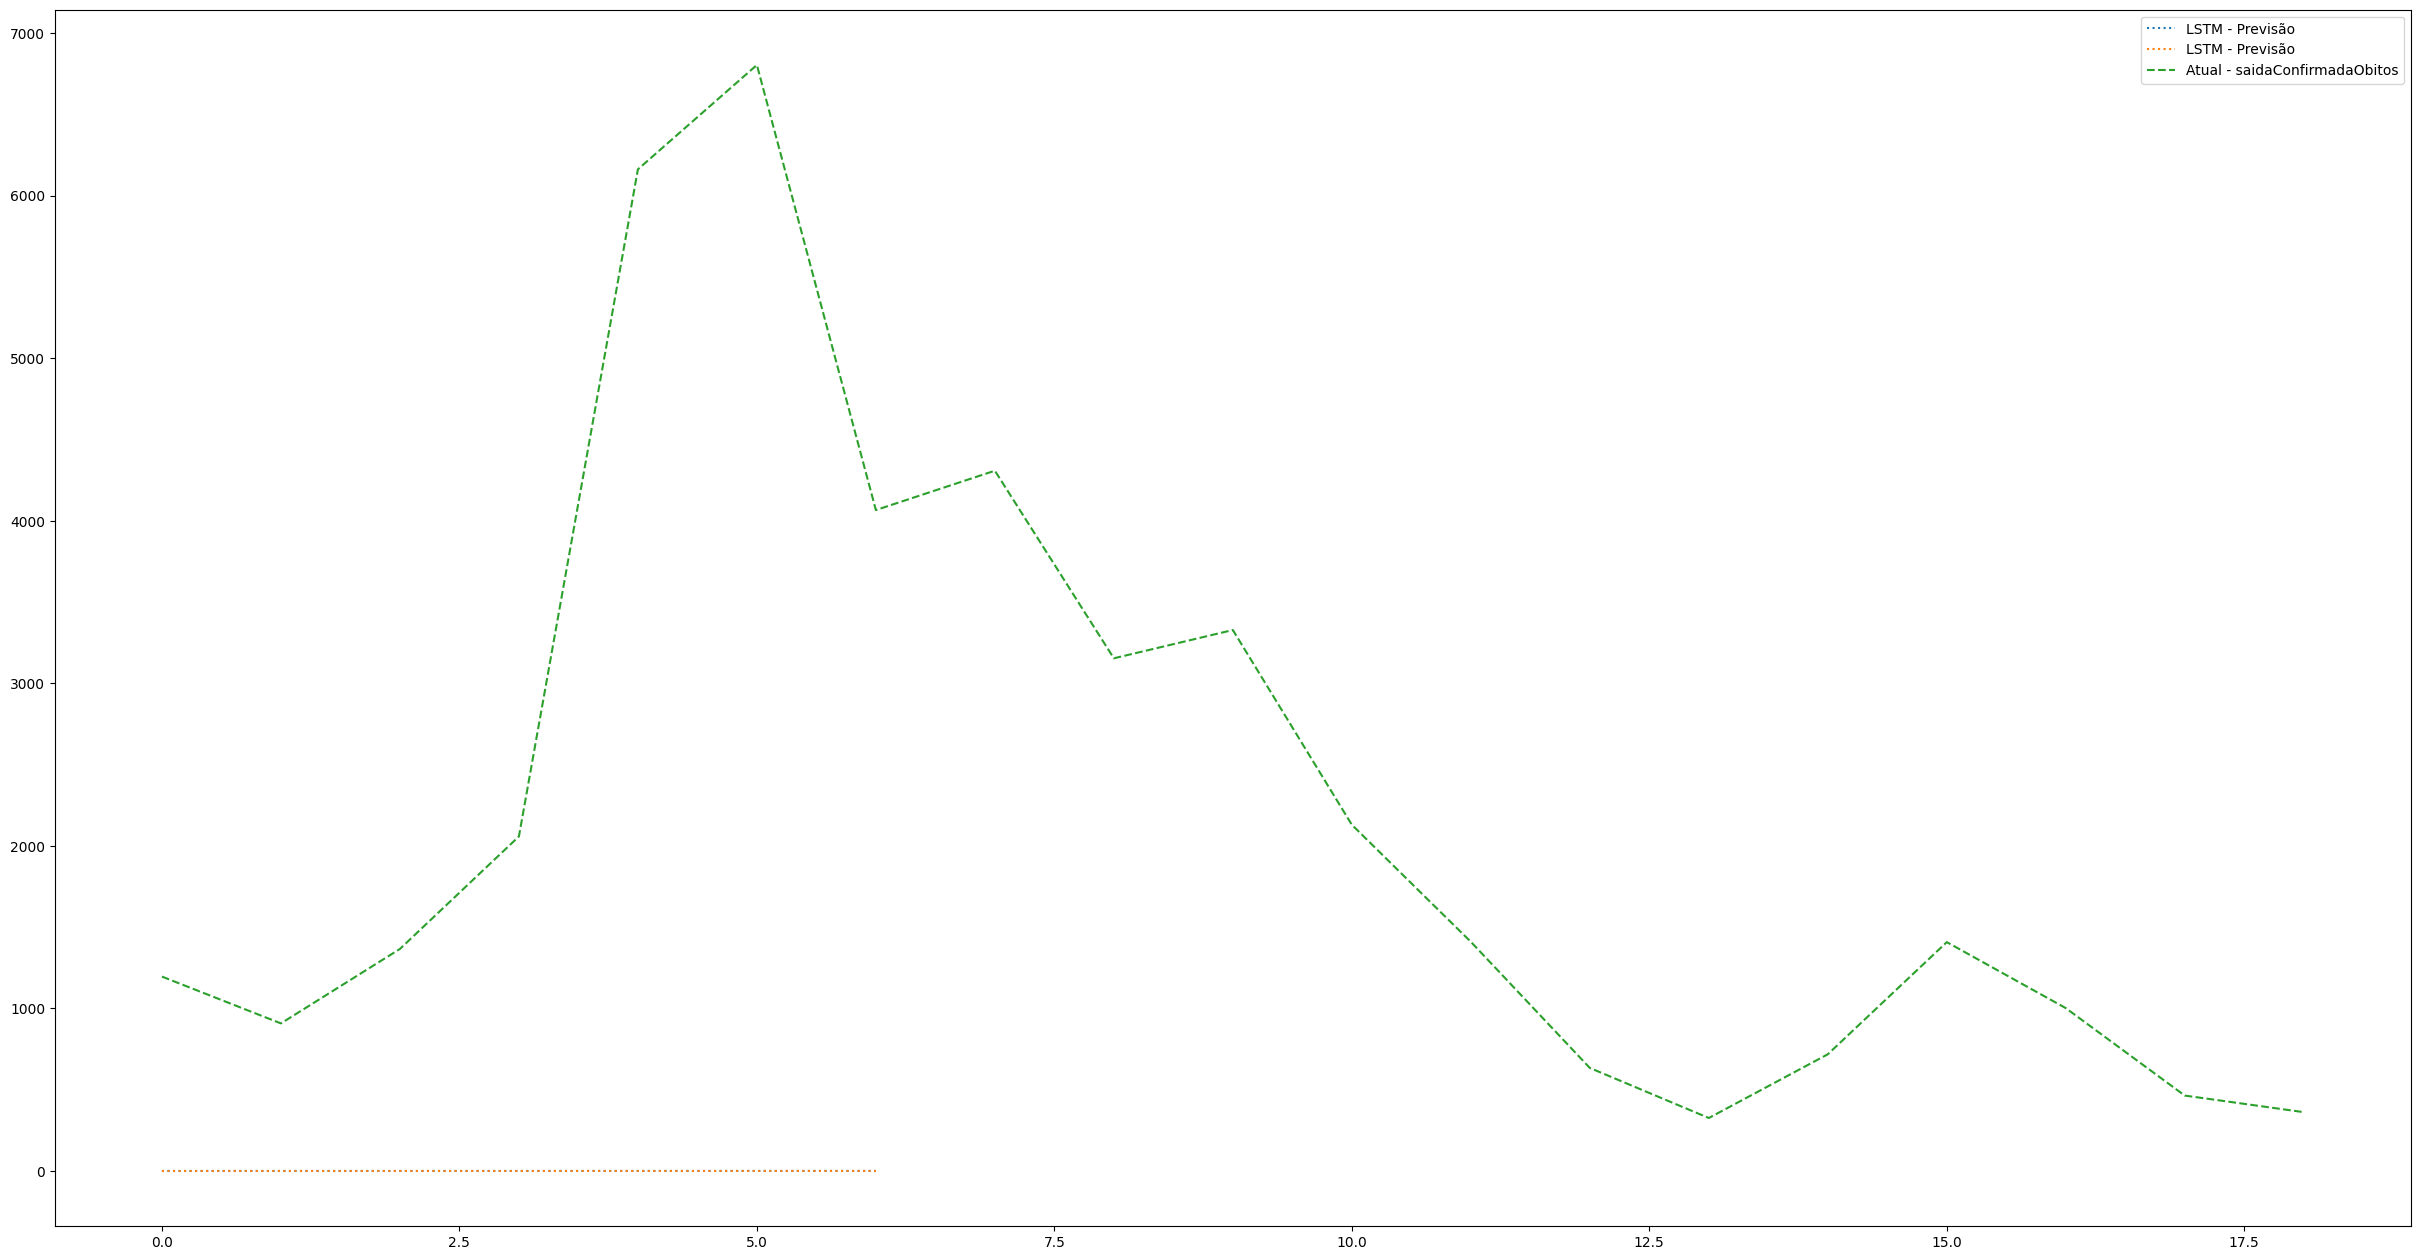
\includegraphics[width=0.99\linewidth]{fig/ModeloLSTM/predicao.png}
    \caption{Gráfico gerado na fase de predição da LSTM}
    \label{fig:enter-label43}
\end{figure}